\documentclass[11pt,a4paper]{article}
\usepackage[margin=2cm]{geometry}
\usepackage[T1]{fontenc}
\usepackage{lmodern}
\usepackage{amsmath}
\usepackage{graphicx}
\usepackage{booktabs}
\usepackage{array}
\usepackage[font=small,labelfont=bf]{caption}
\usepackage[hidelinks]{hyperref}
\usepackage{microtype}
\usepackage{siunitx}
\sisetup{range-phrase=--, range-units=single}
\setlength{\parskip}{0.25em}

\title{\vspace{-1.2cm}\textbf{Concerted Li-ion migration in Li$_{10}$GeP$_2$S$_{12}$ with a universal equivariant potential: PES validation and MD statistics of concerted events}}
\author{[Author name] \\ \small Final project, Introduction to Materials Informatics, Skoltech}
\date{\small October 2026}

\begin{document}
\maketitle
\vspace{-0.6cm}

\begin{abstract}
\noindent Fast Li transport in the superionic conductor Li$_{10}$GeP$_2$S$_{12}$ (LGPS) proceeds by concerted migration of several Li ions with a DFT barrier of \SI{0.20}{eV}, much lower than the \SI{0.47}{eV} single-ion energy landscape. Universal machine-learning interatomic potentials (uMLIPs) make nanosecond molecular dynamics (MD) of such materials affordable, but whether they reproduce concerted migration has not been tested. Using the equivariant uMLIP SevenNet-0, we (1) computed climbing-image NEB profiles for vacancy-assisted migration of $n=1$--4 Li ions along the $c$-channel and (2) counted concerted events in a single \SI{300}{ps} NVT trajectory at \SI{700}{K} with the directed-graph method. SevenNet gives a symmetric four-ion concerted barrier of \SI{0.15}{eV} (25\% below DFT), forward barriers $\le$\SI{0.09}{eV} for all other paths, and no stable end state for an isolated single-ion hop, i.e.\ a softened PES. In MD, 83\% of Li hops belong to concerted events (\SI{3.0}{events\per ps}, mean size 3.9 ions); the Haven ratio $H_R=0.41$ agrees with the directed-graph estimate (0.43) and with the AIMD correlation factor of 3.0, and the event-size distribution decays monotonically without the shoulder at $3<n<8$ reported for a trained MLIP.
\end{abstract}

\section{Introduction}
Solid electrolytes are required for all-solid-state Li batteries, and LGPS is one of the few Li superionic conductors (SICs) with liquid-like room-temperature conductivity, $\sim$\SI{12}{mS\,cm^{-1}}~\cite{Kamaya2011}. He, Zhu and Mo showed by ab initio MD (AIMD) and DFT nudged elastic band (NEB) calculations that fast diffusion in SICs does not occur through isolated hops but through concerted migration of several ions: in LGPS four Li ions on Li1/Li3 sites move simultaneously along the $c$-channel with a barrier of \SI{0.20}{eV}, whereas the energy landscape felt by a single ion has a barrier of \SI{0.47}{eV}; the AIMD correlation factor at \SI{900}{K} is 3.0, i.e.\ two to three ions hop together on average~\cite{He2017}. Correlated multi-ion motion was also identified in garnets~\cite{Burbano2016,Kozinsky2016}, and theory and simulations relate ionic motion to mobile-ion interactions, lattice vibrations and anion dynamics~\cite{Rodin2022,Rodin2025,Gordiz2019,Jun2024}.

Statistics of concerted events require long MD runs: AIMD is limited to a few hundred atoms and sub-ns times, which makes diffusional properties statistically uncertain~\cite{He2018}, and small cells introduce finite-size effects~\cite{Grasselli2022}. Machine-learning potentials remove this bottleneck: a PaiNN potential trained on DFT gave 40-ns MD of LGPS and linked its non-Arrhenius behaviour to a Li-sublattice transition near \SI{400}{K}~\cite{Winter2023}, and an MLIP revealed a collective six-ion ring mechanism in LiF~\cite{DeAngelis2026}. Sato \textit{et al.} recently proposed a directed-graph model that reconstructs concerted events from MD trajectories and showed for MLIP-MD of LGPS at \SI{700}{K} that more than three ions frequently move together along $c$~\cite{Sato2026}. Universal MLIPs (uMLIPs) trained on the Materials Project~\cite{Jain2013}, such as the equivariant message-passing network SevenNet~\cite{Park2024,Batzner2022,Schutt2018}, could make such studies possible without training a material-specific model. However, uMLIPs systematically soften the potential energy surface (PES)~\cite{Deng2025}, and this may distort exactly the Li--Li interactions that lower the concerted barrier.

\textbf{Problem.} It is unknown whether a uMLIP reproduces (i) the PES of concerted vacancy-assisted Li migration and (ii) the statistics of concerted events in LGPS. \textbf{Aims.} (1) Benchmark SevenNet-0 NEB profiles for single and concerted migration against DFT~\cite{He2017}; (2) count concerted events in one trajectory at one temperature and compare with the literature~\cite{He2017,Sato2026}.

\section{Methods}
\textbf{Structure and potential.} The ordered tetragonal LGPS cell (Li$_{10}$Ge(PS$_6$)$_2$, $P4_2mc$, 50 atoms, $a=\SI{8.788}{\angstrom}$, $c=\SI{12.658}{\angstrom}$, $E_{\rm hull}=\SI{0.030}{eV/atom}$) was taken from the Materials Project~\cite{Jain2013} (entry mp-696128) and used without further relaxation. All calculations used the pretrained universal potential SevenNet-0 (\texttt{7net-0}, package \texttt{sevenn} 0.11.2)~\cite{Park2024}, an E(3)-equivariant message-passing network of the NequIP type~\cite{Batzner2022} trained on Materials Project relaxation trajectories (MPtrj; checkpoint \texttt{SevenNet\_0\_\_11Jul2024}: 5 interaction layers, 128 channels, $l_{\max}=2$, \SI{5}{\angstrom} cutoff with 8 Bessel radial basis functions, \num{842623} parameters, 89 elements), through ASE 3.26~\cite{Larsen2017} on CPU (PyTorch 2.5.1). No fine-tuning was performed.

\textbf{NEB benchmark (aim 1).} \textit{(A) Idealized $c$-channel.} In a $2\times1\times2$ supercell (200 atoms) the most populated Li column along $c$ (8 Li, spacing 3.06--\SI{3.27}{\angstrom}) was identified and one Li was removed (199 atoms). For $n=1$--4, the $n$ channel Li next to the vacancy were each shifted by one site toward it ($n=1$: single-ion hop; $n\ge2$: concerted migration). End points were relaxed with BFGS to $F_{\max}=\SI{0.02}{eV/\angstrom}$ (at most 400 steps). The NEB used 7 intermediate images, IDPP interpolation and the improved-tangent method; FIRE was run to \SI{0.10}{eV/\angstrom}, then the climbing image~\cite{Henkelman2000} was switched on and run to \SI{0.05}{eV/\angstrom}. \textit{(B) Events taken from MD.} For events detected in the trajectory (below), structure A is the quenched snapshot at the start of the event and B the same snapshot with only the event ions moved to their positions after $\tau$, quenched (BFGS, \SI{0.02}{eV/\angstrom}). A pair was accepted if every event ion moved $>\SI{1.0}{\angstrom}$ and no other Li moved $>\SI{0.7}{\angstrom}$ between A and B; up to 15 candidates spread over the trajectory were tried for each $n=1$--4. The NEB settings were the same as in (A). Reported are $E_{\rm fwd}=E_{\max}-E_{\rm A}$, $E_{\rm bwd}=E_{\max}-E_{\rm B}$, $\Delta E=E_{\rm B}-E_{\rm A}$ and the kinetically resolved barrier $E_{\rm KRA}=E_{\max}-(E_{\rm A}+E_{\rm B})/2$.

\textbf{Molecular dynamics (aim 2).} NVT MD of the $2\times1\times2$ supercell (200 atoms, 80 Li, $17.58\times8.79\times\SI{25.32}{\angstrom^3}$; initial virial pressure \SI{0.18}{GPa}) was run at \SI{700}{K} with the Bussi stochastic velocity-rescaling thermostat~\cite{Bussi2007} ($\tau_T=\SI{100}{fs}$), time step \SI{2}{fs}, Maxwell--Boltzmann initial velocities (seed 42), \SI{10}{ps} equilibration and \SI{300}{ps} production; frames were saved every \SI{50}{fs} (6001 frames), single precision. The \SI{2}{fs} step was validated by NVE runs (\SI{5}{ps}) with 1 and \SI{2}{fs}: total-energy drift $<\SI{0.001}{meV\,atom^{-1}\,ps^{-1}}$ in both. The run took \SI{0.49}{s/step} on 8 CPU cores ($\approx$\SI{20}{h}). Positions were unwrapped by the minimum-image displacement between consecutive frames (valid at constant volume~\cite{vonBulow2020}) after removing the framework drift; the tracer diffusivity $D^*$ was fitted to the Li mean squared displacement (MSD) for lag times of 10--\SI{150}{ps}~\cite{Rapaport2004}, the collective diffusivity $D_\sigma=N_{\rm Li}D_{\rm com}$ was fitted to the MSD of the Li centre of mass (5--\SI{100}{ps}), giving the Haven ratio $H_R=D^*/D_\sigma$ (uncertainty from three \SI{100}{ps} blocks); the relative standard deviation of $D^*$ was estimated from the effective number of hops, ${\rm RSD}=3.43/\sqrt{N_{\rm eff}}+0.04$, $N_{\rm eff}=\max({\rm TMSD})/a^2$, $a=\SI{2.8}{\angstrom}$~\cite{He2018}.

\textbf{Concerted-event detection.} We implemented the directed-graph model of Ref.~\cite{Sato2026}. The trajectory is cut into non-overlapping windows of length $\tau$; a Li whose displacement within a window exceeds $d_{\rm hop}$ is a hop (graph node). A directed edge $j\to i$ is added if the end point of hop $j$ lies within $r_{\rm cut}$ of the start point of hop $i$. Maximal simple paths are enumerated by depth-first search; among paths sharing $>50\%$ of nodes only the longest is kept. A path with net displacement $<r_{\rm cut}$ is a closed loop and is excluded. The event size $n$ is the number of ions in a path ($n=1$: isolated hop; $n\ge2$: concerted event). Following Ref.~\cite{Sato2026}, $\tau=\SI{2.35}{ps}$ is the shortest window in which about half of the Li hop, and $r_{\rm cut}=\SI{2.0}{\angstrom}$ is shorter than the Li--Li nearest-neighbour distance (mode \SI{3.03}{\angstrom}). The main threshold $d_{\rm hop}=\SI{1.8}{\angstrom}$ separates the intra-site vibrational peak from the hop tail of the displacement distribution (Fig.~\ref{fig:events}a); the value of Ref.~\cite{Sato2026}, \SI{1.4}{\angstrom}, is also reported. Robustness was tested on a $3\times3\times3$ grid: $d_{\rm hop}\in\{1.4,1.8,2.2\}$~\AA, $\tau\in\{1.5,2.35,4.0\}$~ps, $r_{\rm cut}\in\{1.6,2.0,2.4\}$~\AA. We report the number of concerted events per ps, the ion-weighted size distribution $P(n)=nN_n/\sum_i iN_i$, the fraction of hops in concerted events, and $\sigma_{\rm DG}/\sigma_{\rm NE}=\langle n_{\rm paths}\rangle D_{\rm corr}/(N_{\rm Li}D^*)$ with $D_{\rm corr}=\langle|\mathbf R_{\rm fin}-\mathbf R_{\rm init}|^2\rangle/6\tau$ over transport paths~\cite{Sato2026}, an estimate of the inverse Haven ratio. All scripts, input structures, settings files, the MD trajectory and raw outputs are available at \url{https://github.com/kisalubitkrovostok-pixel/lgps-concerted-migration-umlip} (Appendix~B).

\section{Results and discussion}
\textbf{PES of concerted migration.} Figure~\ref{fig:neb}a and Table~\ref{tab:neb} show the SevenNet NEB profiles. The four-ion path is the only one with physically equivalent end points ($\Delta E=0$, ions displaced by 2.1--\SI{2.5}{\angstrom}) and corresponds to the typical LGPS concerted mode of Ref.~\cite{He2017}. Its barrier, \SI{0.15}{eV}, is 25\% lower than the DFT value of \SI{0.20}{eV}. For $n=2$ and 3, the shifted end points relax to configurations \SI{0.15}{eV} lower in energy in which the ions move only 1.4--\SI{1.75}{\angstrom} instead of a full site; the forward barriers are $\le\SI{0.03}{eV}$. For $n=1$, the shifted Li relaxed back to its initial site (shift \SI{0.05}{\angstrom}), so SevenNet has no stable end state for an isolated vacancy hop, and the \SI{0.47}{eV} single-ion landscape of DFT could not be reproduced. Of the candidates taken from MD, only two single-ion hops passed the isolation test, and both are partial rather than full site-to-site hops: the relaxed end point lies only 1.6--\SI{1.9}{\angstrom} from the initial position. They give $E_{\rm KRA}=0.063$ and \SI{0.068}{eV} (Fig.~\ref{fig:neb}b). None of the 40 multi-ion candidates ($n=2$--4) passed the isolation test: in 39 of them spectator Li moved by 0.8--\SI{2.6}{\angstrom} on quenching, and in one an event ion relaxed back. Concerted events in MD therefore involve relaxation of the surrounding Li sublattice and cannot be reduced to an isolated $n$-ion path. All SevenNet barriers lie below the DFT references, which is consistent with the systematic PES softening of uMLIPs~\cite{Deng2025}. The softening affects the single-ion landscape more strongly than the concerted barrier, so the qualitative DFT picture, a concerted barrier lower than the single-ion landscape, is not reproduced.

\begin{figure}[t]
\centering
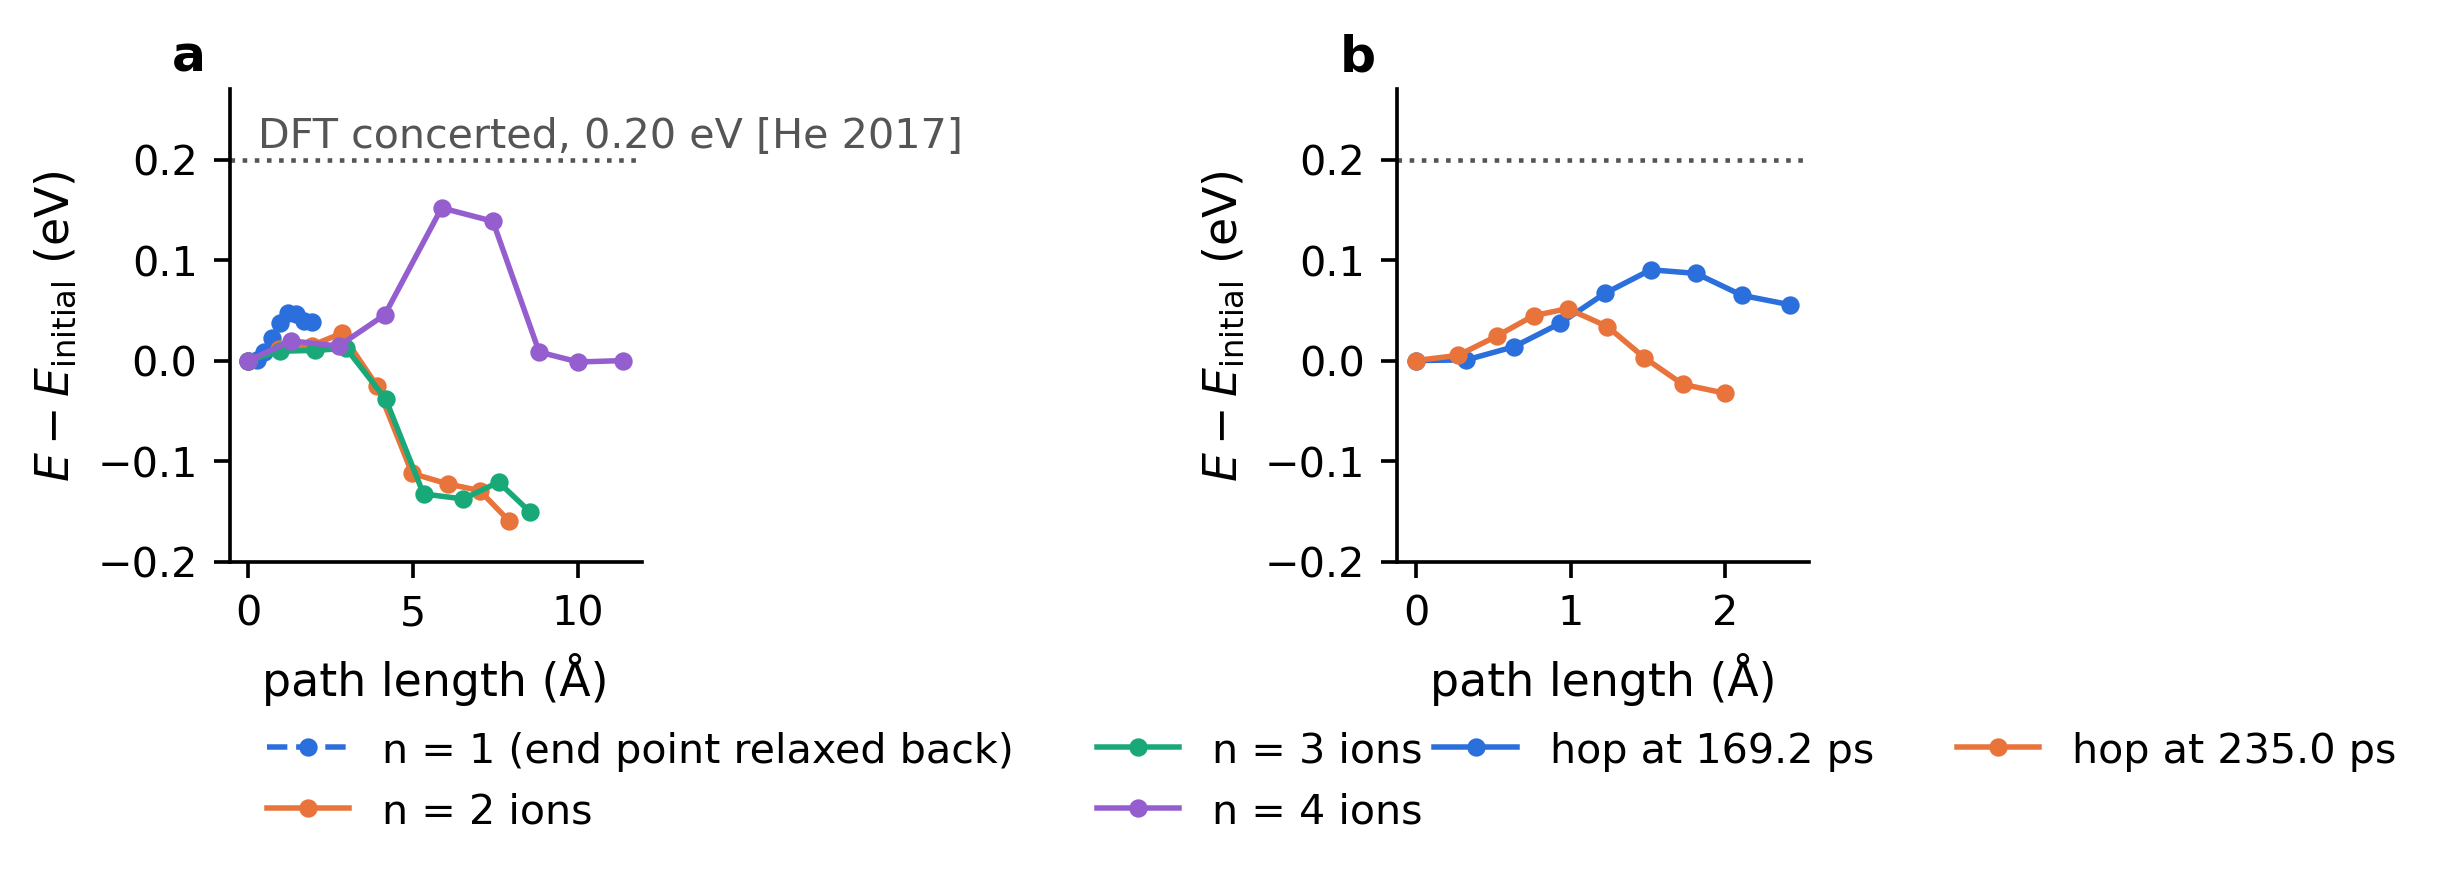
\includegraphics[width=\textwidth]{figures/fig1_neb.png}
\caption{SevenNet-0 CI-NEB energy profiles in LGPS. (a) Vacancy-assisted migration of $n=1$--4 Li ions along the $c$-channel ($2\times1\times2$ supercell, one Li vacancy). For $n=1$ the end point relaxed back to the initial state. Dotted line: DFT concerted barrier~\cite{He2017}. (b) Single-ion hops taken from the \SI{700}{K} MD trajectory.}
\label{fig:neb}
\end{figure}

\begin{table}[t]
\centering
\footnotesize\setlength{\tabcolsep}{4pt}
\caption{Migration barriers (eV). Shift: displacement of the moving ions between the relaxed end points.}
\label{tab:neb}
\begin{tabular}{lccccc}
\toprule
Path & $E_{\rm fwd}$ & $E_{\rm bwd}$ & $\Delta E$ & shift (\AA) & DFT~\cite{He2017} \\
\midrule
$n=1$, idealized & 0.047 & 0.009 & 0.038 & 0.05$^a$ & 0.47 (landscape) \\
$n=2$, idealized & 0.027 & 0.187 & $-0.160$ & 1.41, 1.75 & -- \\
$n=3$, idealized & 0.012 & 0.162 & $-0.150$ & 1.38--1.73 & -- \\
$n=4$, idealized & 0.152 & 0.152 & 0.000 & 2.06--2.49 & 0.20 (concerted) \\
$n=1$, from MD ($t=169.2$ ps) & 0.090 & 0.035 & 0.055 & 1.92 & -- \\
$n=1$, from MD ($t=235.0$ ps) & 0.052 & 0.084 & $-0.033$ & 1.59 & -- \\
\bottomrule
\end{tabular}\\[2pt]
{\footnotesize $^a$ end point relaxed back to the initial state.}
\end{table}

\textbf{Li transport in MD.} The trajectory is stable ($\langle T\rangle=700\pm40$~K, no drift of $E_{\rm pot}$; Appendix~A). The Li MSD is linear (Fig.~\ref{fig:msd}a) and gives $D^*=\SI{2.5e-5}{cm^2\,s^{-1}}$ with an estimated RSD of 9\% ($N_{\rm eff}\approx4500$)~\cite{He2018}. Diffusion is anisotropic: per Cartesian direction, $D_c=\SI{3.7e-5}{cm^2\,s^{-1}}$ along the channel and $D_{ab}=\SI{1.9e-5}{cm^2\,s^{-1}}$ in the $ab$ plane. This is consistent with the substantial $ab$-plane diffusion found in LGPS above the $\approx$\SI{400}{K} Li-sublattice transition~\cite{Winter2023}.

\begin{figure}[t]
\centering
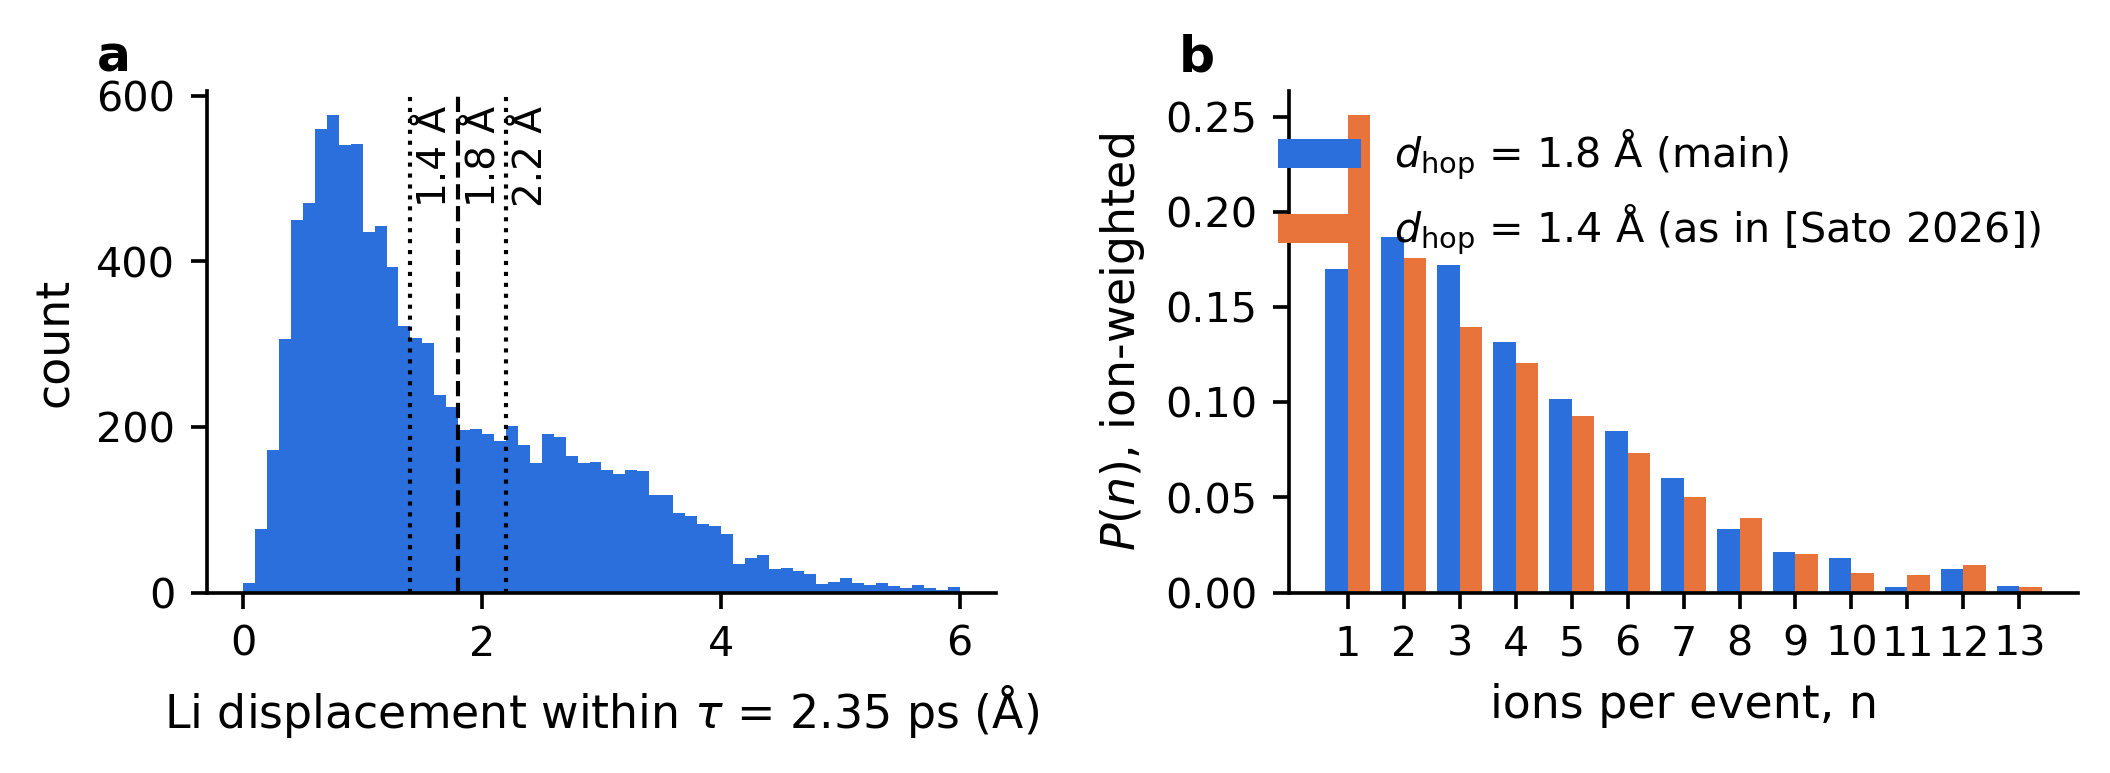
\includegraphics[width=\textwidth]{figures/fig2_events.png}
\caption{Concerted-event statistics, SevenNet-0, \SI{700}{K}, \SI{300}{ps}. (a) Li displacement within non-overlapping windows $\tau=\SI{2.35}{ps}$; vertical lines mark the tested hop thresholds $d_{\rm hop}$. (b) Ion-weighted distribution of event size $n$ for the main threshold and for the threshold used in Ref.~\cite{Sato2026} ($\tau=\SI{2.35}{ps}$, $r_{\rm cut}=\SI{2.0}{\angstrom}$).}
\label{fig:events}
\end{figure}

\begin{figure}[t]
\centering
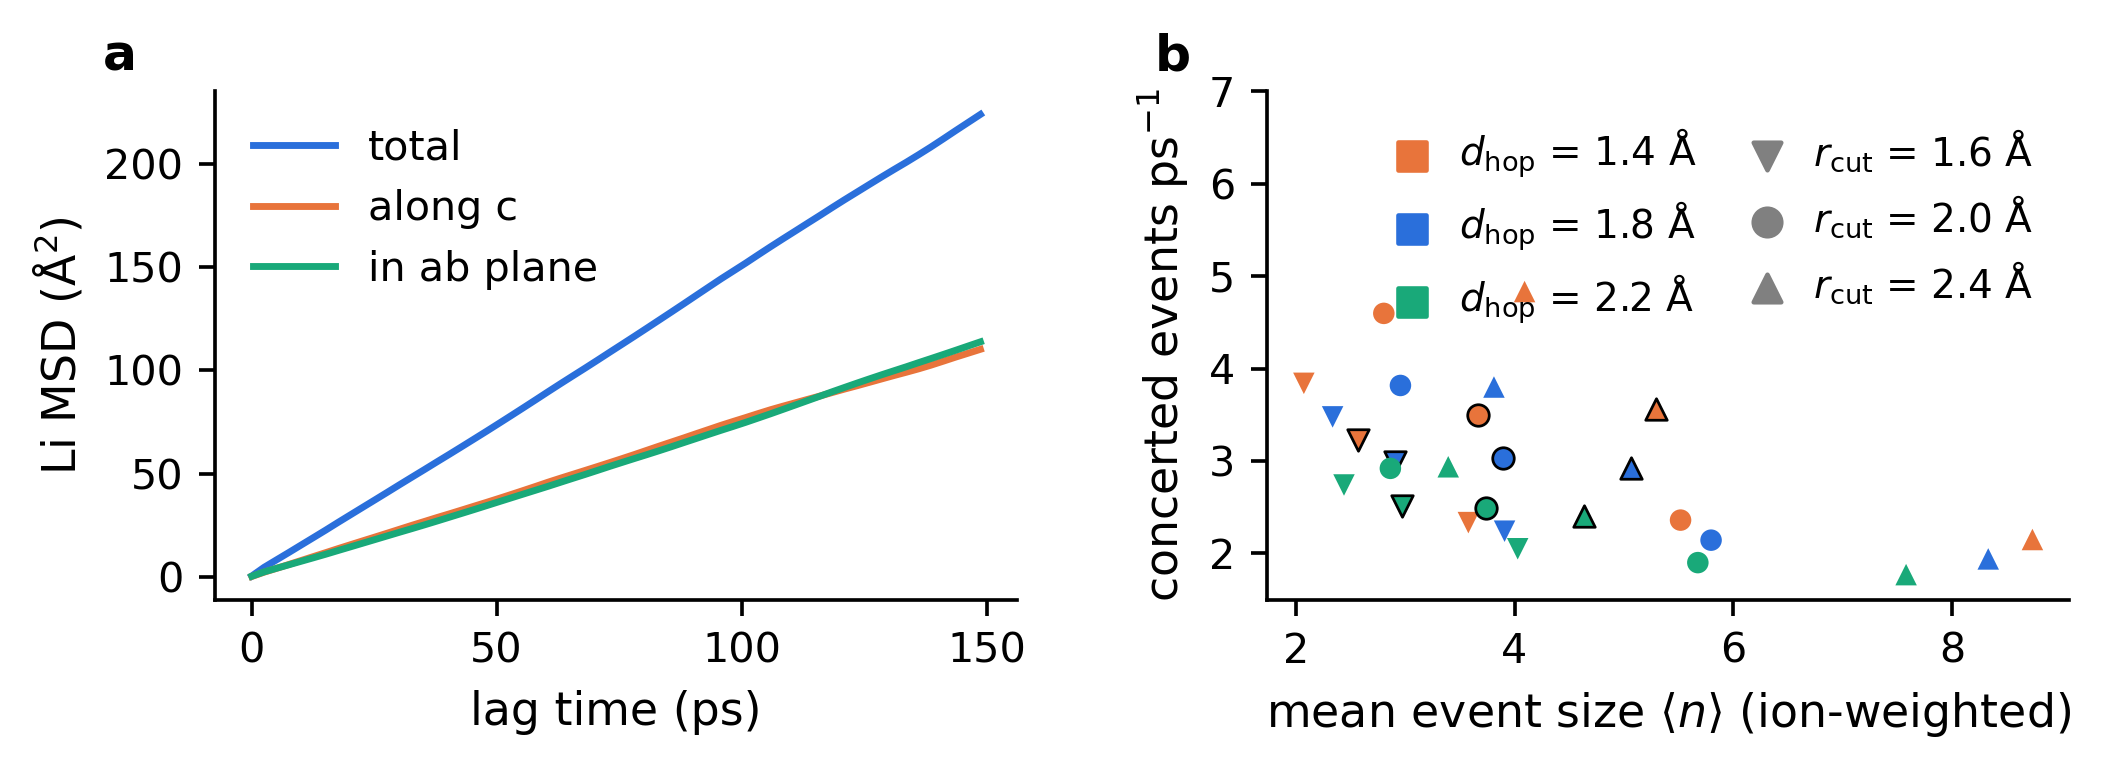
\includegraphics[width=\textwidth]{figures/fig3_msd_scan.png}
\caption{(a) Li mean squared displacement: total and components along $c$ and in the $ab$ plane. (b) Sensitivity of concerted-event statistics to the detection parameters (27 combinations). Colour: $d_{\rm hop}$; marker: $r_{\rm cut}$; black edge: $\tau=\SI{2.35}{ps}$, no edge: $\tau=1.5$ or \SI{4.0}{ps}.}
\label{fig:msd}
\end{figure}

\textbf{Concerted events.} With the main parameters, the trajectory contains 3790 hops grouped into 1556 events, 905 of which are concerted ($n\ge2$), i.e.\ \SI{3.0}{events\per ps} in the 80-Li cell (Table~\ref{tab:events}). Most hops (83\%) belong to concerted events, the ion-weighted mean size is 3.9 ions (2.5 per event), and events with up to 13 ions occur (Fig.~\ref{fig:events}b). With the threshold of Ref.~\cite{Sato2026} ($d_{\rm hop}=\SI{1.4}{\angstrom}$), more small displacements count as hops: 1044 concerted events (\SI{3.5}{ps^{-1}}), 75\% of hops concerted, mean size 3.7. Over all 27 parameter combinations the rate varies between 1.8 and \SI{4.8}{ps^{-1}}, the concerted fraction between 0.51 and 0.95, and the mean size between 2.1 and 8.7 (Fig.~\ref{fig:msd}b). Longer $\tau$ and larger $r_{\rm cut}$ merge hops into fewer, larger events. The absolute number of events is therefore defined only together with the detection parameters. The conclusion that most hops are concerted holds for all 27 combinations.

\begin{table}[t]
\centering
\footnotesize\setlength{\tabcolsep}{4pt}
\caption{Concerted-migration statistics in LGPS: this work vs.\ literature.}
\label{tab:events}
\begin{tabular}{lcc>{\raggedright\arraybackslash}p{4.3cm}}
\toprule
 & This work, main & This work, $d_{\rm hop}=1.4$ \AA & Literature \\
\midrule
Method, $T$, length & \multicolumn{2}{c}{SevenNet-0 MD, 700 K, 300 ps, 200 atoms} & \\
Concerted events ($n\ge2$) & 905 (3.0 ps$^{-1}$) & 1044 (3.5 ps$^{-1}$) & not reported \\
Hops in concerted events & 83\% & 75\% & dominant mechanism~\cite{He2017} \\
Mean size (ion-weighted) & 3.9 & 3.7 & 2--3 ions (AIMD, 900 K)~\cite{He2017} \\
$\sigma_{\rm DG}/\sigma_{\rm NE}$ & 2.3 & 2.6 & corr.\ factor 3.0 (AIMD, 900 K)~\cite{He2017} \\
Haven ratio $H_R$ & \multicolumn{2}{c}{0.41 direct (blocks 0.23--0.62); 0.43 = $(\sigma_{\rm DG}/\sigma_{\rm NE})^{-1}$} & $<1$ at high $T$ (MLIP)~\cite{Winter2023} \\
$P(n)$ shape & \multicolumn{2}{c}{monotonic decay; $P(4\le n\le7)=0.38$ / 0.34} & shoulder, $3<n<8$ (MLIP, 700 K)~\cite{Sato2026} \\
$D^*$ (cm$^2$ s$^{-1}$) & \multicolumn{2}{c}{$2.5\times10^{-5}$} & -- \\
\bottomrule
\end{tabular}
\end{table}

\textbf{Comparison with the literature.} Neither reference reports an absolute event rate, so we compare intensive measures (Table~\ref{tab:events}). The direct Haven ratio, $H_R=D^*/D_\sigma=0.41$ (block values 0.23--0.62), agrees with the independent directed-graph estimate $(\sigma_{\rm DG}/\sigma_{\rm NE})^{-1}=0.43$, which confirms that the detected events carry the collective transport. The correlation enhancement $\sigma_{\rm DG}/\sigma_{\rm NE}=2.3$--2.6 is close to the correlation factor of 3.0 from AIMD~\cite{He2017}, and $H_R<1$ agrees with the strongly correlated high-temperature regime found with a trained MLIP~\cite{Winter2023}; the remaining difference is within the expected temperature trend, since correlations weaken on cooling~\cite{Winter2023}, and within the parameter spread of Fig.~\ref{fig:msd}b. Large events are frequent, as in the MLIP study of Ref.~\cite{Sato2026}: $P(4\le n\le7)=0.34$--0.38. However, our distribution decays monotonically after its maximum at $n=1$--2, whereas Ref.~\cite{Sato2026} reports a shoulder at $3<n<8$. Sato \textit{et al.} attribute this shoulder possibly to periodic images in their $\approx$400-atom cell~\cite{Sato2026}; our cell is even smaller, so the absence of the shoulder is more plausibly due to the softer SevenNet PES, which lets single ions hop more easily (Table~\ref{tab:neb}). Only 45\% of concerted events have their net displacement within $37^\circ$ of $c$ (50\% for single hops), so in this model concerted motion is not restricted to the $c$-channel.

\textbf{Significance and limitations.} SevenNet-0 reproduces the qualitative picture of fast, highly correlated Li transport in LGPS at a cost of one CPU-day per \SI{300}{ps}, but with a softened PES: the four-ion barrier is 25\% too low and the single-ion landscape is missing. Rates and diffusivities from this model should therefore be regarded as upper bounds, and fine-tuning on DFT NEB images is needed before quantitative use. The main limitations are: (i) the SevenNet NEB paths were not recomputed with DFT, so the comparison relies on the published barriers~\cite{He2017}, which were obtained in a different vacancy and occupation setting; (ii) the 200-atom cell may enhance correlations through periodic images~\cite{Grasselli2022,Sato2026}, and the neutral-vacancy model ignores defect charge effects~\cite{Freysoldt2014}; (iii) one trajectory of \SI{300}{ps}, shorter than the planned \SI{0.5}{ns}, at a single temperature above the sublattice transition, with a fixed Materials Project lattice; (iv) event counts depend on $d_{\rm hop}$, $\tau$ and $r_{\rm cut}$ (Fig.~\ref{fig:msd}b).

\section{Conclusion}
We tested whether the universal equivariant potential SevenNet-0 reproduces concerted vacancy-assisted Li migration in LGPS. (1) The PES is softened. The four-ion concerted barrier is \SI{0.15}{eV}, 25\% below the DFT value of \SI{0.20}{eV}; all other forward barriers are below \SI{0.1}{eV}; and an isolated single-ion hop has no stable end state, so the DFT hierarchy (single-ion landscape \SI{0.47}{eV} $>$ concerted \SI{0.20}{eV}) is lost. (2) One \SI{300}{ps} trajectory at \SI{700}{K} contains 905 concerted events (\SI{3.0}{ps^{-1}}, 83\% of all hops, mean size 3.9 ions), with $D^*=\SI{2.5e-5}{cm^2\,s^{-1}}$ and a Haven ratio of 0.41, consistent with the directed-graph estimate (0.43) and with the AIMD correlation factor of 3.0. The size distribution, however, lacks the large-event shoulder reported for a trained MLIP. A uMLIP captures that Li transport in LGPS is concerted but not the energetics that control it, so DFT-level fine-tuning is required for quantitative studies of collective ion transport.

\begin{thebibliography}{99}
\small
\setlength{\itemsep}{0pt}
\bibitem{Kamaya2011} N.~Kamaya \textit{et al.}, A lithium superionic conductor, \textit{Nat. Mater.} \textbf{10}, 682 (2011).
\bibitem{He2017} X.~He, Y.~Zhu, Y.~Mo, Origin of fast ion diffusion in super-ionic conductors, \textit{Nat. Commun.} \textbf{8}, 15893 (2017).
\bibitem{Burbano2016} M.~Burbano, D.~Carlier, F.~Boucher, B.~J.~Morgan, M.~Salanne, Sparse cyclic excitations explain the low ionic conductivity of stoichiometric Li$_7$La$_3$Zr$_2$O$_{12}$, \textit{Phys. Rev. Lett.} \textbf{116}, 135901 (2016).
\bibitem{Kozinsky2016} B.~Kozinsky \textit{et al.}, Effects of sublattice symmetry and frustration on ionic transport in garnet solid electrolytes, \textit{Phys. Rev. Lett.} \textbf{116}, 055901 (2016).
\bibitem{Rodin2022} A.~Rodin, K.~Noori, A.~Carvalho, A.~H.~Castro Neto, Microscopic theory of ionic motion in solids, arXiv:2111.02849 (2022).
\bibitem{Rodin2025} A.~Rodin, B.~A.~Olsen, A.~Ustyuzhanin, A.~Maevskiy, Time-local stochastic equation of motion for solid ionic electrolytes, arXiv:2504.06595 (2025).
\bibitem{Gordiz2019} K.~Gordiz, S.~Muy, W.~G.~Zeier, Y.~Shao-Horn, A.~Henry, Enhancement of ion diffusion by targeted phonon excitation, arXiv:1911.07492 (2019).
\bibitem{Jun2024} K.~Jun, B.~Lee, R.~L.~Kam, G.~Ceder, The nonexistence of a paddlewheel effect in superionic conductors, \textit{Proc. Natl. Acad. Sci. USA} \textbf{121}, e2316493121 (2024).
\bibitem{He2018} X.~He, Y.~Zhu, A.~Epstein, Y.~Mo, Statistical variances of diffusional properties from ab initio molecular dynamics simulations, \textit{npj Comput. Mater.} \textbf{4}, 18 (2018).
\bibitem{Grasselli2022} F.~Grasselli, Investigating finite-size effects in molecular dynamics simulations of ion diffusion, heat transport, and thermal motion in superionic materials, \textit{J. Chem. Phys.} \textbf{156}, 134705 (2022).
\bibitem{Winter2023} G.~Winter, R.~G\'omez-Bombarelli, Simulations with machine learning potentials identify the ion conduction mechanism mediating non-Arrhenius behavior in LGPS, \textit{J. Phys. Energy} (2023); arXiv:2211.05713.
\bibitem{DeAngelis2026} P.~De~Angelis \textit{et al.}, Exploring lithium diffusion in LiF with machine learning potentials: from point defects to collective ring diffusion, \textit{npj Comput. Mater.} (2026), doi:10.1038/s41524-026-02132-8.
\bibitem{Sato2026} R.~Sato, Y.~Ando, K.~Sau, Y.~Shibuta, Visualizing concerted ion migration of superionic conductors via directed graphs, \textit{Chem. Mater.} \textbf{38}, 287--295 (2026).
\bibitem{Jain2013} A.~Jain \textit{et al.}, The Materials Project: A materials genome approach to accelerating materials innovation, \textit{APL Mater.} \textbf{1}, 011002 (2013).
\bibitem{Park2024} Y.~Park, J.~Kim, S.~Hwang, S.~Han, Scalable parallel algorithm for graph neural network interatomic potentials in molecular dynamics simulations, \textit{J. Chem. Theory Comput.} \textbf{20}, 4857 (2024).
\bibitem{Batzner2022} S.~Batzner \textit{et al.}, E(3)-equivariant graph neural networks for data-efficient and accurate interatomic potentials, \textit{Nat. Commun.} \textbf{13}, 2453 (2022).
\bibitem{Schutt2018} K.~T.~Sch\"utt, H.~E.~Sauceda, P.-J.~Kindermans, A.~Tkatchenko, K.-R.~M\"uller, SchNet -- a deep learning architecture for molecules and materials, \textit{J. Chem. Phys.} \textbf{148}, 241722 (2018).
\bibitem{Deng2025} B.~Deng \textit{et al.}, Systematic softening in universal machine learning interatomic potentials, \textit{npj Comput. Mater.} \textbf{11}, 9 (2025).
\bibitem{Larsen2017} A.~H.~Larsen \textit{et al.}, The atomic simulation environment -- a Python library for working with atoms, \textit{J. Phys.: Condens. Matter} \textbf{29}, 273002 (2017).
\bibitem{Henkelman2000} G.~Henkelman, B.~P.~Uberuaga, H.~J\'onsson, A climbing image nudged elastic band method for finding saddle points and minimum energy paths, \textit{J. Chem. Phys.} \textbf{113}, 9901 (2000).
\bibitem{Bussi2007} G.~Bussi, D.~Donadio, M.~Parrinello, Canonical sampling through velocity rescaling, \textit{J. Chem. Phys.} \textbf{126}, 014101 (2007).
\bibitem{vonBulow2020} S.~von~B\"ulow, J.~T.~Bullerjahn, G.~Hummer, Systematic errors in diffusion coefficients from long-time molecular dynamics simulations at constant pressure, \textit{J. Chem. Phys.} \textbf{153}, 021101 (2020).
\bibitem{Rapaport2004} D.~C.~Rapaport, \textit{The Art of Molecular Dynamics Simulation}, 2nd ed., Cambridge University Press (2004).
\bibitem{Freysoldt2014} C.~Freysoldt \textit{et al.}, First-principles calculations for point defects in solids, \textit{Rev. Mod. Phys.} \textbf{86}, 253 (2014).
\end{thebibliography}

\appendix
\section*{Appendix A. MD stability}
\begin{figure}[h]
\centering
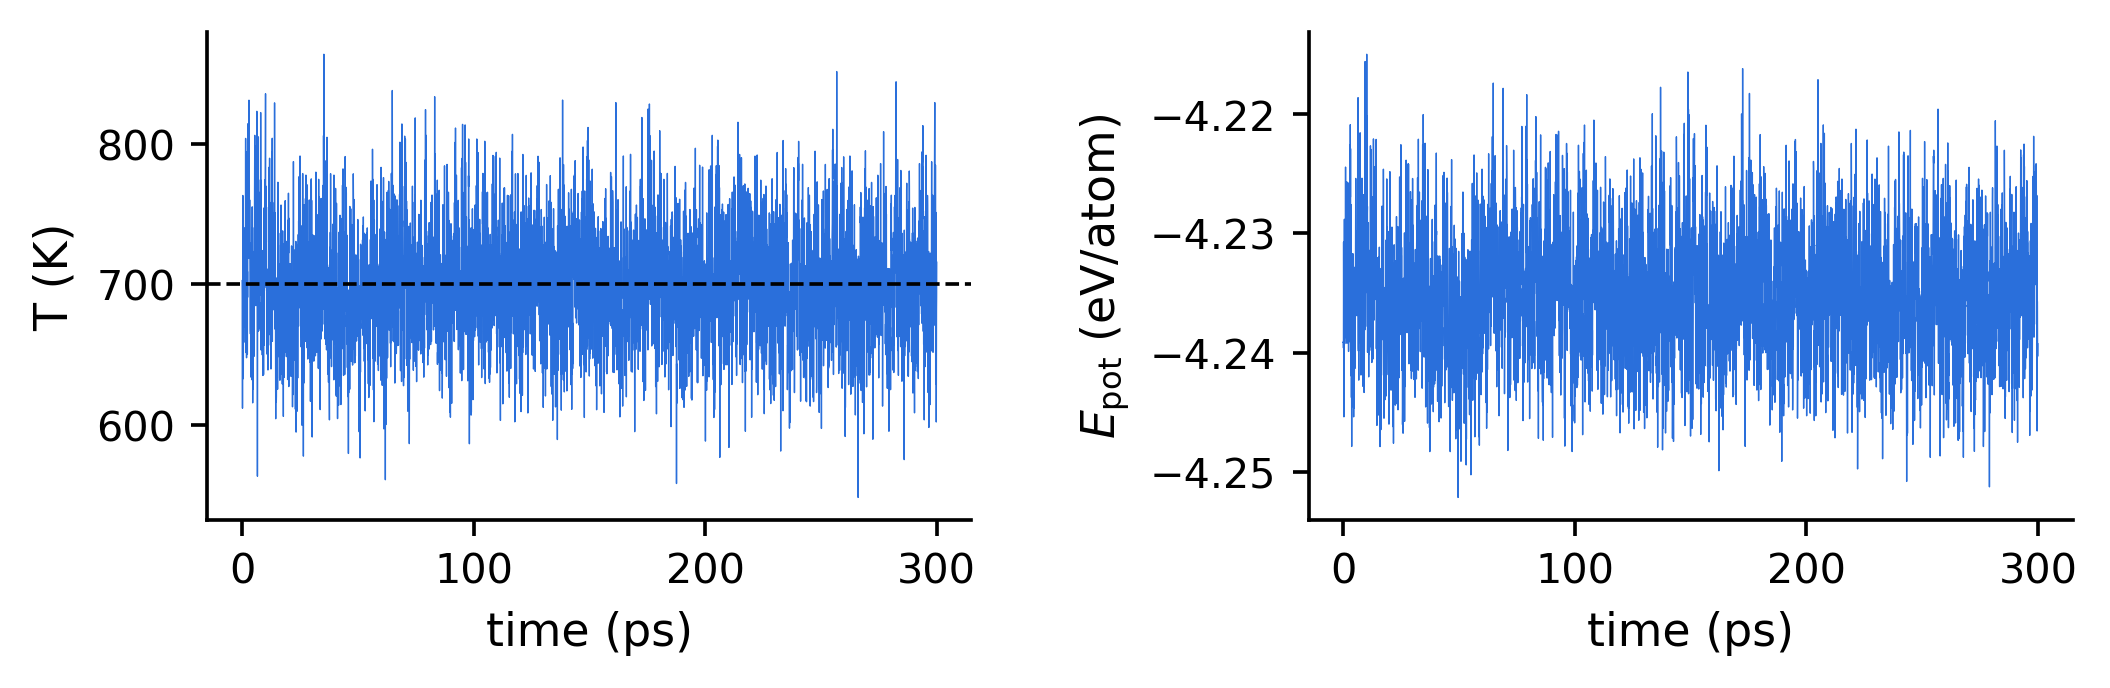
\includegraphics[width=\textwidth]{figures/figA1_md_stability.png}
\caption{Instantaneous temperature and potential energy during the \SI{300}{ps} NVT production run (SevenNet-0, LGPS, \SI{700}{K}).}
\end{figure}

\section*{Appendix B. Reproducibility package}
{\small All files are available at \url{https://github.com/kisalubitkrovostok-pixel/lgps-concerted-migration-umlip}. Paths are relative to the repository root.}\par\smallskip
\footnotesize
\begin{tabular}{lp{7.2cm}}
\toprule
File / folder & Content \\
\midrule
\texttt{05\_structure/LGPS.cif}, \texttt{LGPS\_source.json} & input structure and its Materials Project record \\
\texttt{06\_scripts\_methods/run\_md.py}, \texttt{md.sbatch} & NVT MD (settings in \texttt{04\_data\_MD\_run/settings.json}) \\
\texttt{06\_scripts\_methods/neb\_lgps\_sevennet.py} & idealized $c$-channel NEB (set A) \\
\texttt{06\_scripts\_methods/neb\_from\_md.py} & NEB on events extracted from MD (set B) \\
\texttt{06\_scripts\_methods/concerted\_events.py} & directed-graph event detection and parameter scan \\
\texttt{06\_scripts\_methods/dt\_test\_sevennet.py} & time-step (NVE drift) test \\
\texttt{06\_scripts\_methods/haven\_ratio.py} & direct Haven ratio $D^*/D_\sigma$ \\
\texttt{06\_scripts\_methods/make\_paper\_figures.py} & all figures and the $D^*$/RSD values of this report \\
\texttt{06\_scripts\_methods/environment-sevennet.txt} & exact package versions \\
\texttt{02\_data\_*}, \texttt{03\_data\_NEB}, \texttt{04\_data\_MD\_run} & raw results (event lists, NEB profiles and paths, MD logs) \\
\bottomrule
\end{tabular}

\end{document}
